
The contents of this chapter are published in~\citet{visani_holographic-vae_2024}, under the title
\textit{Holographic-(V)AE: An end-to-end SO(3)-equivariant (variational) autoencoder in Fourier space}.

The appeal of group-equivariant neural networks is straightforward in the supervised learning context,
in which the objective is to fit a function to provided input-output pairs that may contain knwon
group symmetries. Indeed, neural networks equivariant to SO(3) and other euclidean transformations
have advanced the state-of-the-art in many supervised tasks~\citep{weiler_3d_2018, thomas_tensor_2018,
fuchs_se3-transformers_2020, brandstetter_geometric_2022, batzner_e3-equivariant_2022, musaelian_learning_2022,
satorras_en_2022, liao_equiformer_2022}.

In conceiving this work, we hypothesized that applying the group-equivariant paradigm to
unsupervised learning could map out compact representations of data that are agnostic to a specified
symmetry transformation. In the world of unsupervised learning, auto-encoders (AE's) - and their
probabilistic version, variational auto-encoders (VAE's) - are among the most popular popular paradigms,
as they can learn robust and compact representations of high-dimensional data~\cite{kingma_auto-encoding_2013}.

Therefore, in this chapter we apply our SO(3)-equivariant modeling framework to the domain of autoencoders
and develop Holographic-(V)AE (H-(V)AE), an end-to-end SO(3)-equivariant (variational) autoencoder trained
to reconstruct the holographic encoding of data. H-(V)AE learns an SO(3)-equivariant latent space composed
of a \textit{maximally informative} set of invariants and an equivariant frame describing the orientation of
the data.

We extensively test the performance and properties of H-(V)AE in two domains. First, we focus on
spherical images, demonstrating high accuracy in unsupervised classification and clustering
tasks. Second, we focus on proteins, and demonstrate that H-(V)AE can be effectively
used to construct compact, informative, and symmetry-aware representations of protein structures,
which can be used for downstream tasks. Specifically, we leverage H-(V)AE trained on a large corpus
of protein structure neighborhoods to construct local representations of protein-ligand
binding pockets that are both rotationally and translationally equivariant (i.e., SE(3)
equivariant). When combined with a simple Random Forest Regressor, we achieve state-of-the-art
accuracy on the task of  predicting the binding affinity between a protein and a ligand in complex.
Code and pre-trained models are freely available at
\href{https://github.com/gvisani/Holographic-VAE}{https://github.com/gvisani/Holographic-VAE}.

This work can be placed within an increasing literature of group-equivariant representation and unsupervised
learning.

Disentangled from neural networks and data-driven learning, there is a diverse body of literature on
constructing representations of atomic systems that are invariant or equivariant to euclidean symmetries,
leveraging spherical fourier transforms and CG tensor products~\citep{drautz_atomic_2019,
musil_physics-inspired_2021}. Notably,~\citet{uhrin_through_2021} constructs SO(3)-invariant representations
of point clouds using the ZFT and CG tensor product iterations. H-(V)AE can be seen as a data-driven instance
of this framework.

On the data-driven side, several works attempt to learn representations that are invariant to certain classes
of transformations, but avoid equivariant neural networks. \citet{shu_deforming_2018} and 
\citet{koneripalli_rate-invariant_2020} learn general ``shape"
embeddings by learning a separate ``deformation" embedding. However, their networks are not
explicitly equivariant to the transformations of interest.
Other work proposes to learn an exactly invariant embedding alongside an approximate (but not
equivariant) group action to align the input and the reconstructed data. For
example,~\citet{mehr_manifold_2018} learns in quotient space by sampling the group's orbit and
computing the reconstruction loss by taking the infimum over the group. This approach is best
suited for discrete and finite groups, and it is computationally expensive as it is akin to data
augmentation. \citet{lohit_rotation-invariant_2020} construct an SO(3)-invariant autoencoder for
spherical signals by learning an invariant latent space and minimizing a loss which first finds the
rotation that best aligns the true and reconstructed signals, introducing an added optimization
step - potentially very expensive for 3D data - and reconstructing the signals only up to a global
rotation.

A small body of work, which H-(V)AE is most closely related to, focuses on developing equivariant
autoencoders. Several methods construct data and group-specific architectures to auto-encode data
equivariantly, learning an equivariant representation in the process~\citep{hinton_transforming_2011,
kosiorek_stacked_2019}. Others use supervision to extract
class-invariant and class-equivariant representations~\citep{feige_invariant-equivariant_2022}. =
A concurrent theoretical work proposed to train an encoder that encodes elements into an invariant
embedding and an equivariant group action, then using a standard decoder that uses the invariants
to reconstruct the elements in a canonical form, and finally applying the learned group action to
recover the data's original form~\citep{winter_unsupervised_2022}.
Our method in SO(3) is closely related to this work, with the crucial difference that we use an
equivariant decoder and that we learn to reconstruct the Fourier encoding of the data. A more
detailed comparison of the two approaches and the benefits of our fully equivariant approach can be
found in the Appendix (Sec.~\ref{sec:mlp_decoder_appendix}) and in Table~\ref{table:mlp_decoder_comparison}.


\section{Methods}

\noindent {\bf Network architecture and training.}  H-(V)AE consists of an encoder that, through
learned linear projections and pre-set nonlinear operations, project the data  onto a compressed
rotationally equivariant latent space. A trained decoder that is similarly constructed then takes
this latent projection and reconstructs the input data. The combination of leaned linear and
pre-set nonlinear operations form equivariant Clebsch-Gordan blocks (CG bl.) both for the encoder
and the decoder; see Figure~\ref{fig:model} and below for details on the structure of  a
Clebsch-Gordan block. \\

Using the Clebsch-Gordan blocks, we  construct a fully rotationally equivariant architecture for
unsupervised learning. Specifically, the encoder takes as input a steerable tensor with maximum
degree $\ell_\text{max}$ and, via a stack of Clebsch-Gordan blocks, iteratively and equivariantly
transfers information from higher degrees to lower ones, down to the final encoder layer with 
$\ell_\text{max} = 1$, resulting in the invariant ($\ell=0$) and the frame-defining equivariant
($\ell=1$) embeddings.  The frame is constructed by learning two vectors from the $\ell=1$
embedding in the final layer of the encoder and using Gram-Schmidt to find the corresponding
orthonormal basis~\cite{schmidt_zur_1907}. The third orthonomal basis vector is then calculated as
the cross product of the first two.


The decoder learns to reconstruct the input from the invariant ($\ell=0$) embedding of the
encoder's final layer $\mathbf{z}$ and the frame, iteratively increasing the maximum degree
$\ell_\text{max}$ of the intermediate representations by leveraging the CG Tensor Product within
the Clebsch-Gordan blocks (Figure~\ref{fig:model}C). To add stochasticity and make the model
variational (i.e., constructing H-VAE as opposed to H-AE), we parameterize the \textit{invariant}
part of the latent space by an isotropic Gaussian, i.e., we learn two sets of size $z$ invariants,
corresponding to means and standard deviations. \\

We train H-(V)AE to minimize the reconstruction loss $\mathcal{L}_{rec}$ between the original and
the reconstructed tensors, and, for H-VAE only, to minimize the Kullback-Leibler divergence 
$D_{KL}$ of the posterior invariant latent space distribution $q(\vz|\vx)$ from the selected prior
$p(\vz)$~\cite{kingma_auto-encoding_2013}:
\begin{equation}
    \mathcal{L}(\vx, \vx') = \alpha \mathcal{L}_{\text{rec}}(\vx, \vx') + \beta D_{KL}(q(\vz|\vx) || p(\vz))
    \label{eqn:training_objective}
\end{equation}
We use mean square error (MSE) for $\mathcal{L}_{\text{rec}}$, which as we show in
Section~\ref{sec:pairwise_inv_rec_loss}, respects the necessary property of SO(3) pairwise
invariance, ensuring that the model remains rotationally equivariant. We cast an isotropic normal
prior to the invariant latent space: $p(\vz) = \mathcal{N}(\bf 0, \mI)$. Hyperparameters $\alpha$
and $\beta$ control the trade-off between reconstruction accuracy and latent space
regularization~\cite{higgins_beta-vae_2022}; see Section~\ref{sec:training_objective_hyperparams}
for details on tuning of these rates during training.\\



As a result of this training, H-(V)AE learns a \textit{disentangled} latent space consisting of a
maximally informative invariant ($\ell = 0$) component $\mathbf{z}$ of arbitrary size, as well as
three orthonormal vectors ($\ell = 1$), which represent the global 3D orientation of the object and
reflect the {\em coordinate frame} of the input tensor. Crucially, the disentangled nature of the
latent space is respected at all stages of training, and is guaranteed by the model's rotational
equivariance; see Figure~\ref{fig:disentanglement_mnist} for a visual example. We discuss the
equivariant properties of H-(V)AE in more detail in Figure~\ref{fig:canonical_frames_1,7}, and
empirically verify the equivariance of our model up to numerical errors in
Table~\ref{table:equivariance_error}.\\

\noindent {\bf Invariant Conditioning.}
Since all of a datapoint's invariant information is compressed in one latent embedding
$\mathbf{z}$, it is trivial to condition the latent space with invariant properties of the data.
This process can be used to exclude the properties' information from the latent embedding, thereby
allowing the model to focus on more nuanced characteristics, or to allow for conditional generation
if training with a variational objective~\citep{sohn_learning_2015}. In our model, we apply
conditioning by first linearly projecting the conditioning so that its dimentionality matches that
of $\mathbf{z}$, then adding it to $\mathbf{z}$ before and feeding the result into the decoder.


\noindent {\bf Architecture of a Clebsch-Gordan block.} 
Each Clebsch-Gordan block (CG bl.) consists of a trained linear layer ({\em Linearity} (Lin)), an
efficient tensor product (ETP) to inject nonlinearity in the network, and normalization steps by
{\em Batch Norm} (BN) and {\em Signal Norm} (SN) (see Section~\ref{sec:layers}). We found using
batch norm alone often caused activations to explode in the decoder during inference, and
introduced signal norm to counteract this effect. While training with signal norm alone is stable,
we found keeping both norms to speed up convergence in preliminary experiments
(Fig.~\ref{fig:training_loss_trace_H-AE}). \\

\begin{figure*}[t!]
    \centering
    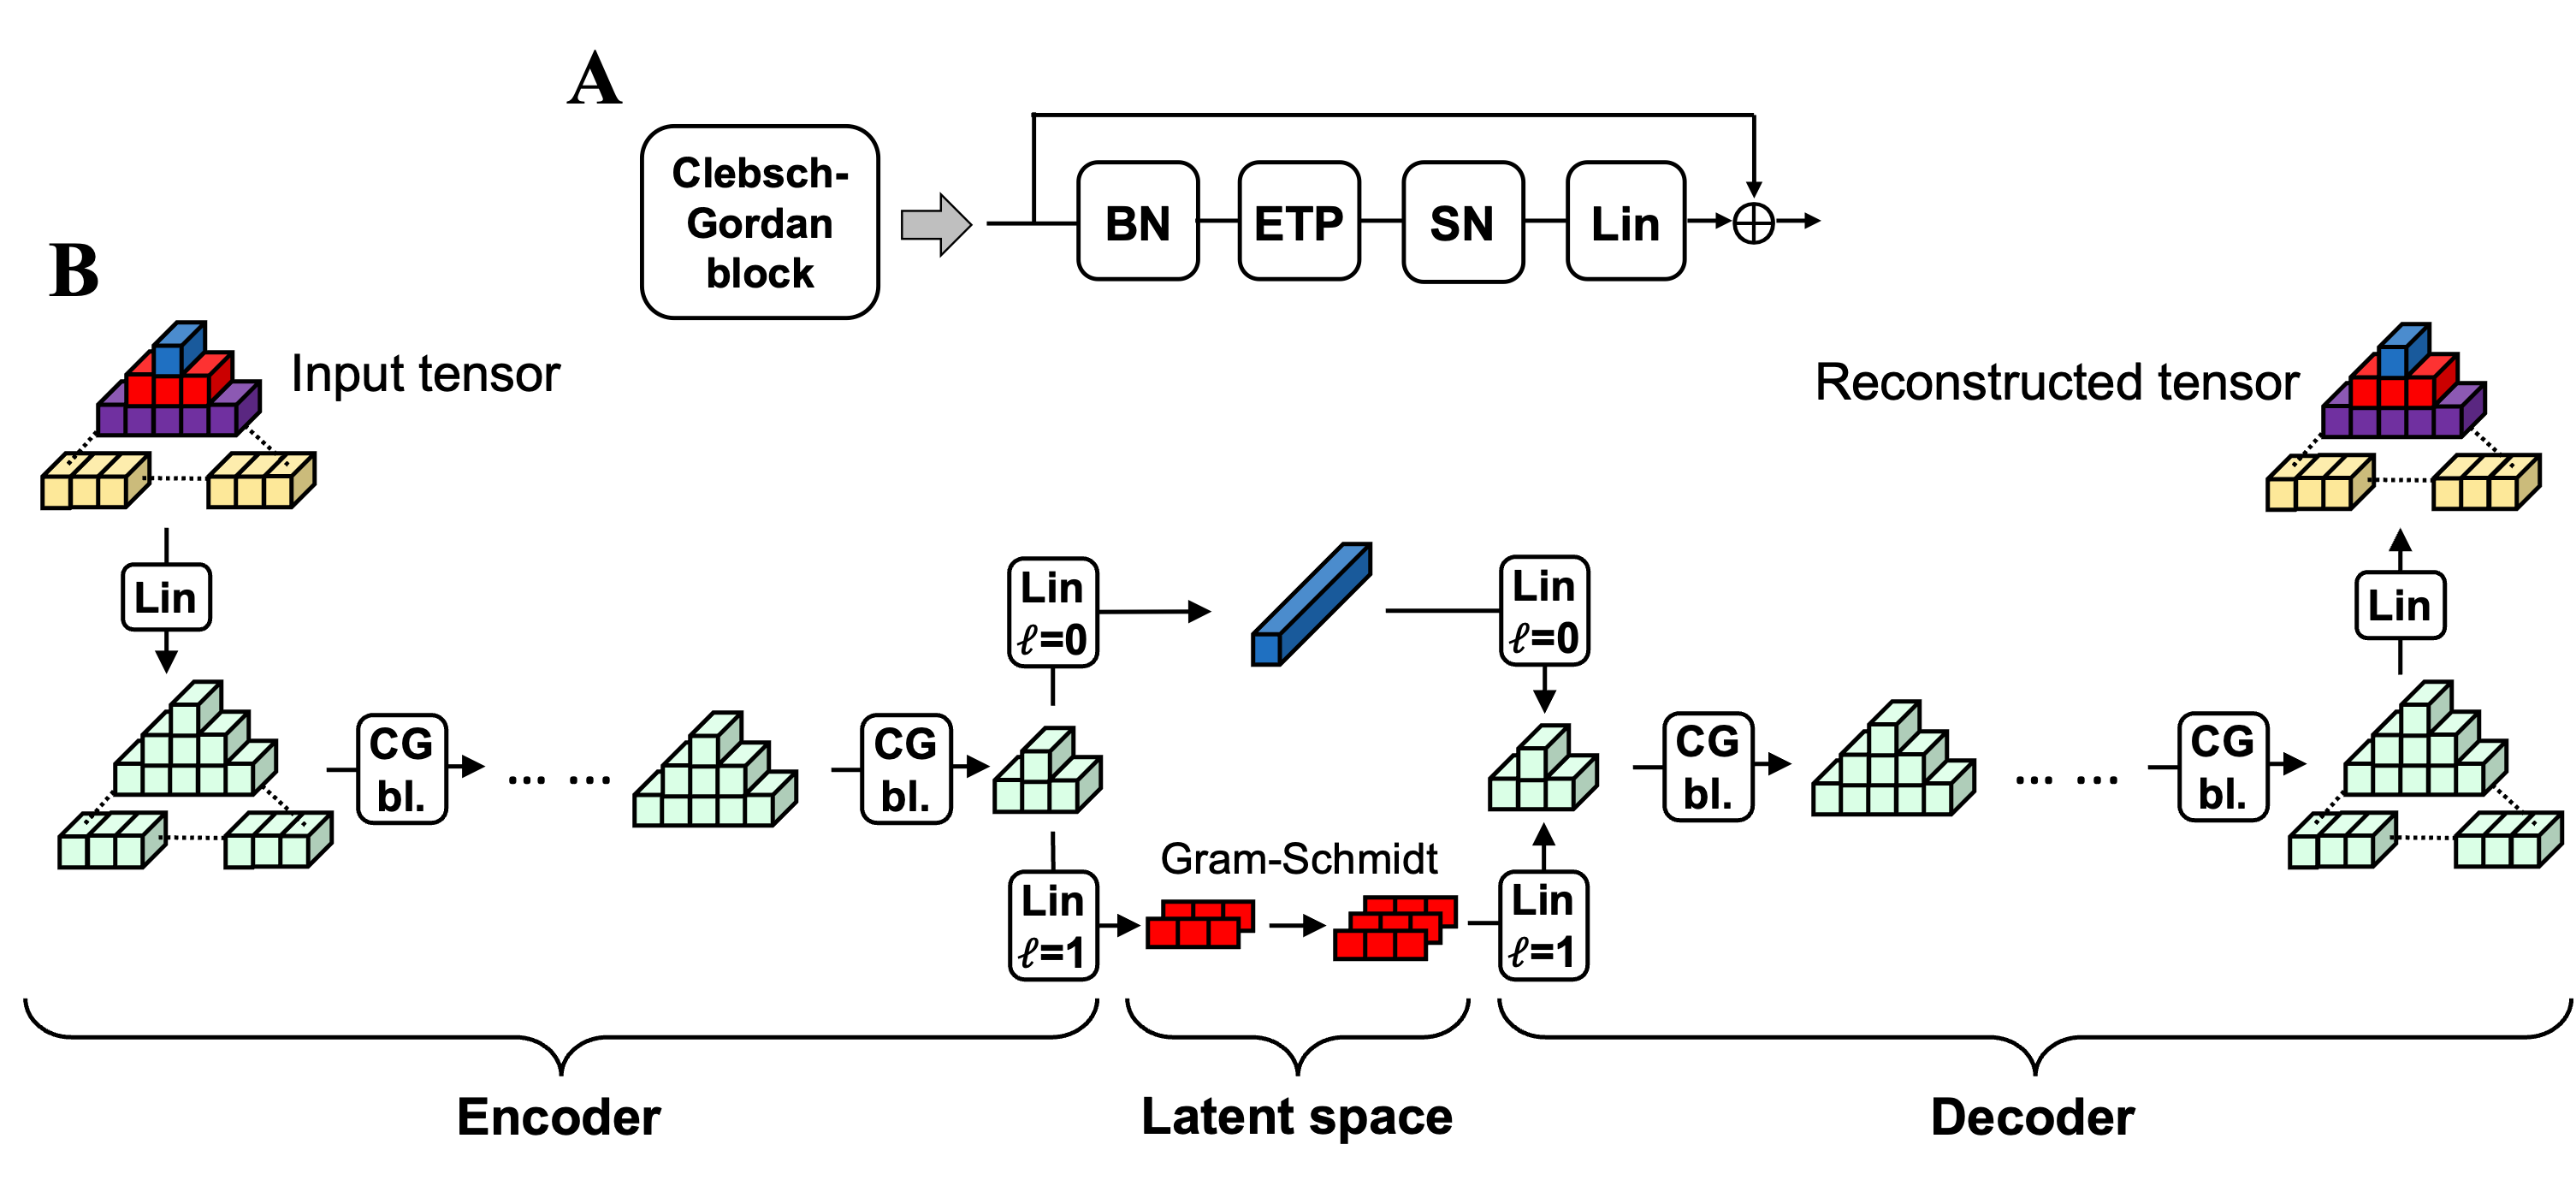
\includegraphics[width=0.9\textwidth]{figures/hvae_for_quals.png}
    \figcaption{Visualization of H-(V)AE's architecture.}{}
    \medskip
    \small
    \justifying
    \textbf{A:} Schematic of a Clebsch-Gordan Block (CG bl.), with batch norm (BN), efficient
    tensor product (ETP), and signal norm (SN), and Linear (Lin) operations. \textbf{B:} Schematic
    of the H-AE architecture. We color-code features of different degrees in the input and in the
    latent space for clarity. The H-VAE schematic differs only in the latent space, where two sets
    of invariants are learned (means and standard deviations of an isotropic Gaussian distribution).
    \label{fig:model}
\end{figure*}

\begin{figure*}[htbp]
    \centering
    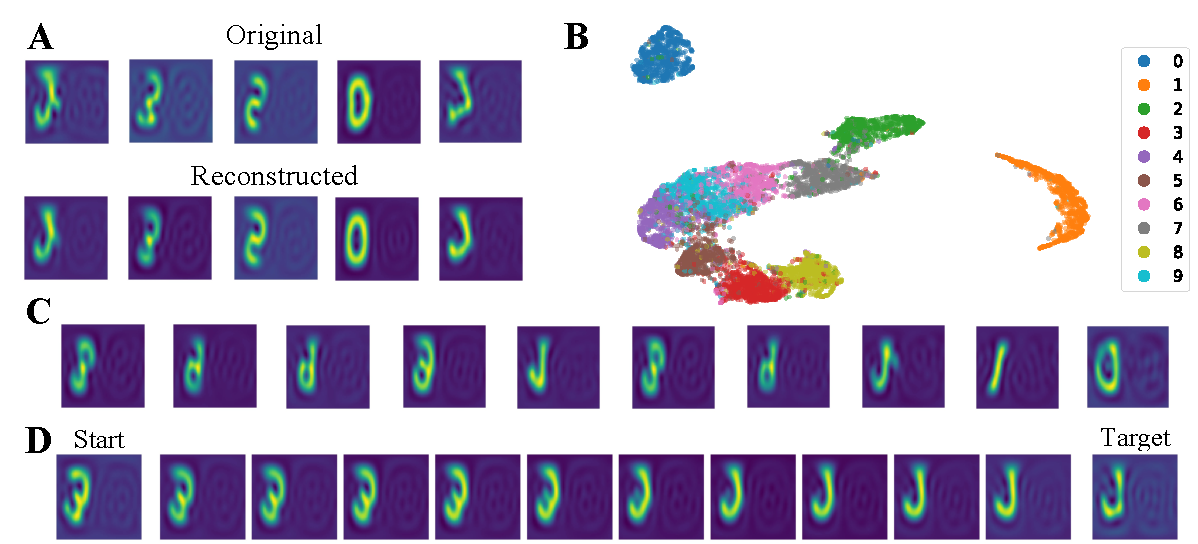
\includegraphics[width=0.83\textwidth]{figures/figure2_beta=0.6.pdf}
    \figcaption{H-VAE on MNIST-on-the-sphere.}{}
    \medskip
    \small
    \justifying
    Evaluation on rotated digits for an H-VAE trained on non-rotated digits with $z = 16$.
    \textbf{(A)} Original and reconstructed images in the canonical frame after inverse transform
    from Fourier space. The images are projected onto a plane. Distortions at the edges and
    flipping are side-effects of the projection. \textbf{(B)} visualization of the latent space via
    2D UMAP~\cite{mcinnes_umap_2020}. Data points are colored by digit identity. \textbf{(C)}
    Random images generated by feeding the decoder invariant embeddings sampled from the prior
    distribution and the canonical frame. See more examples in
    Figure~\ref{fig:mnist_samples_VAE_z_16_beta_0pt6}. \textbf{(D)} Example image trajectory by
    linearly interpolating through the learned invariant latent space.
    Interpolated invariant embeddings are fed to the decoder alongside the canonical frame. . See
    more examples in Figure~\ref{fig:mnist_trajectories_VAE_z_16_beta_0pt6}. MNIST-on-the-sphere
    dataset is created by projecting data from the planar MNIST on a discrete unit sphere, using
    the Driscoll-Healey (DH) method with a bandwidth (bw) of 30~\cite{cohen_spherical_2018}.
    \label{fig:mnist_viz}
\end{figure*}


\begin{figure*}
    \centering
    \resizebox{0.5\textwidth}{!}{
    \begin{tabular}{c}
        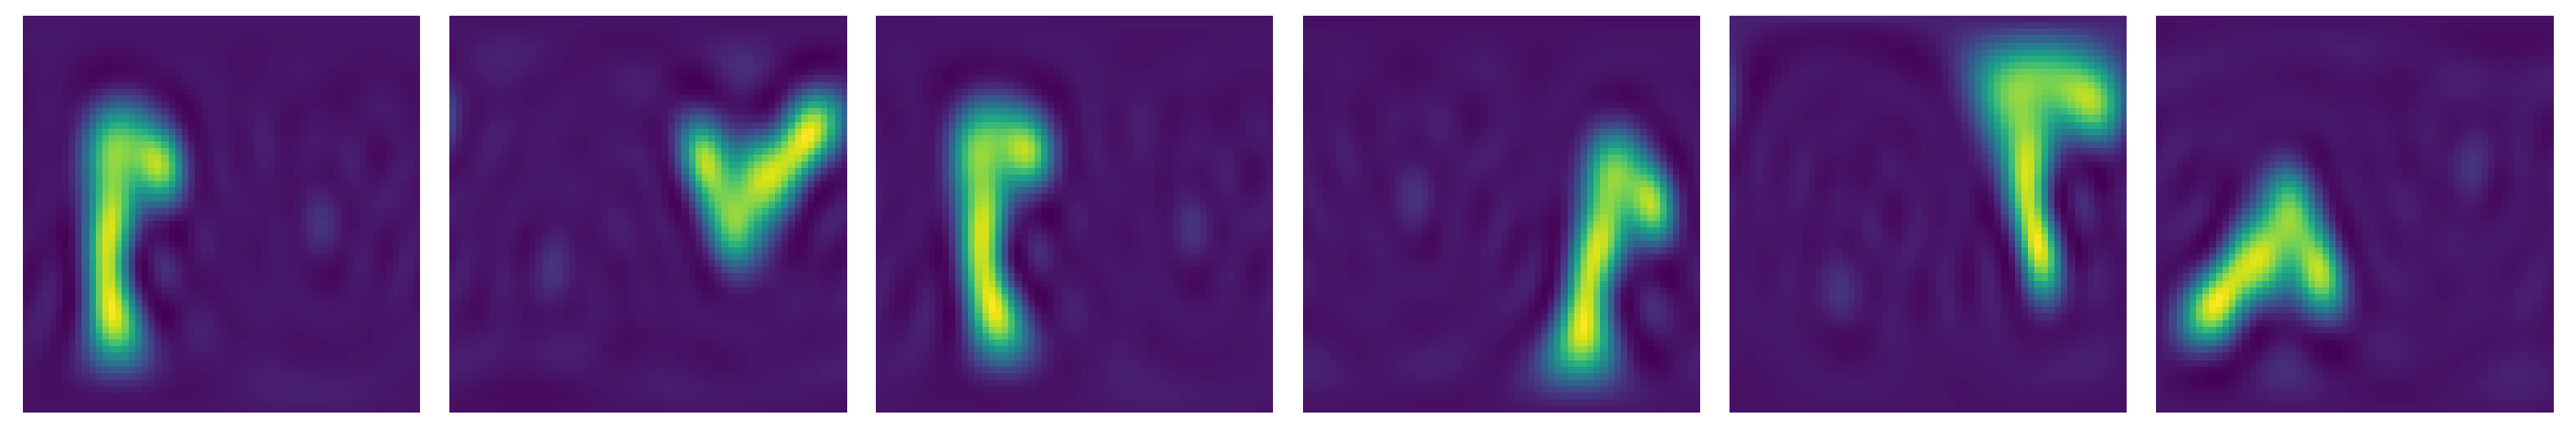
\includegraphics[width=0.8\textwidth]{figures/mnist/disentanglement/disentanglement-n_samples=1-seed=4.pdf}
        \\
        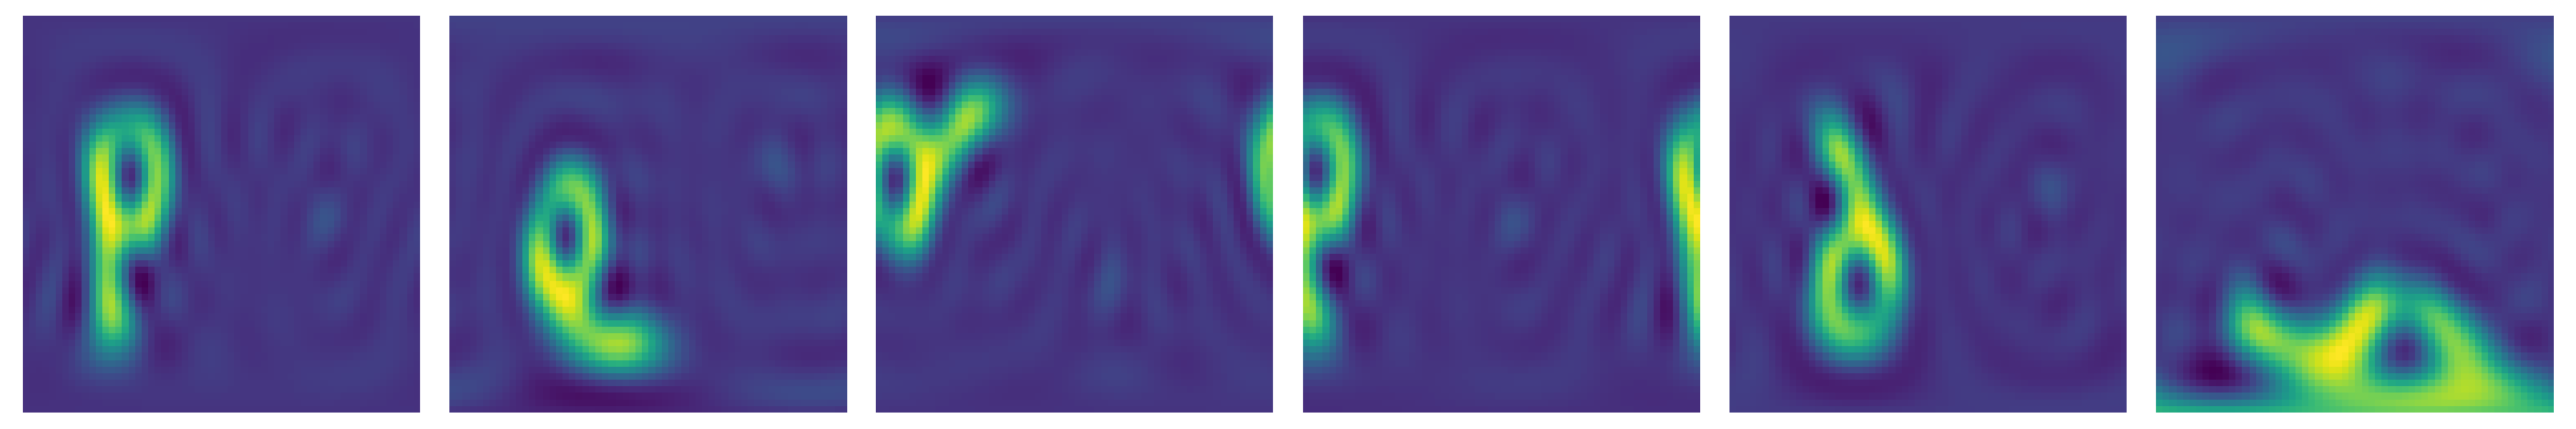
\includegraphics[width=0.8\textwidth]{figures/mnist/disentanglement/disentanglement-n_samples=1-seed=5.pdf}
        \\
        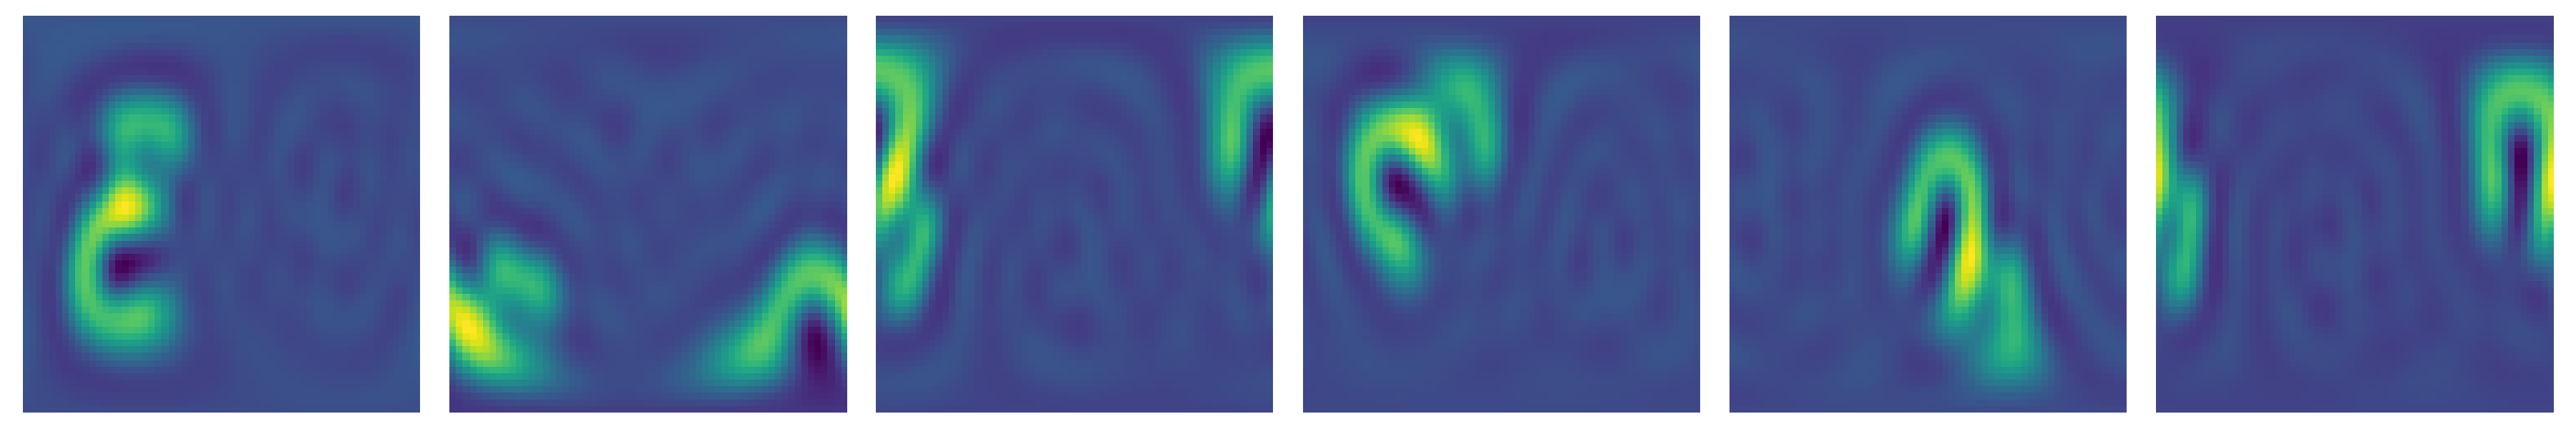
\includegraphics[width=0.8\textwidth]{figures/mnist/disentanglement/disentanglement-n_samples=1-seed=7.pdf}
    \end{tabular}
    }
    \figcaption{Visual evidence of the disentanglement in the latent space of
    MNIST-on-the-sphere.}{}
    \medskip
    \small
    \justifying
    For each row, the invariant embedding $\mathbf{z}$ is held fixed, and a different frame (i.e.,
    the rotation matrix) is used. Frames are sampled randomly and differ across rows, with the
    exception of the first column, where the frame is the same. Then, $\mathbf{z}$ and the frame
    are fed to the decoder and the Inverse Fourier Transform is used to generate the reconstructed
    spherical image, which is projected onto a plane for the ease of visualization. Modulo the
    distortions given by projecting the image onto a plane, it is clear that the invariant
    embedding contains all semantic information, and the frame solely determines the orientation of
    the image.
    \label{fig:disentanglement_mnist}
\end{figure*}


\section{Results}

\subsection{Rotated MNIST on the sphere}
\label{sec:mnist_results}
We extensively test the performance of  H-(V)AE on the MNIST-on-the-sphere
dataset~\cite{deng_mnist_2012}. Following ref.~\cite{cohen_spherical_2018}, we project the MNIST
dataset, which includes images of handwritten numbers,  onto the lower hemisphere of a discrete
unit sphere.
We consider two variants of training/test set splits, NR/R and R/R, differing in whether the
training/test images have been randomly rotated (R) or not (NR). For each dataset, we map the
images to steerable tensors via the Zernike Fourier Transform (ZFT) in Eq.~\ref{eq:ZFT} and train
models with different different sizes of latent spaces ($z=16$ vs. $z=120$) and model
types (AE vs. VAE). In all cases the model architecture follows from Figure~\ref{fig:model}C.\\
\\
For variational models, we tune the regularization strength $\beta$ such as to maximize
the expected quality of generated samples. We define samples to be of high quality if they 1) can
be correctly classified by a classifier trained on real data, and 2) if they are diverse enough,
finding that there is a trade-off between the two. We assess sample quality across $\beta$ by
generating them with conditional models and computing the accuracy of a classifier trained on real
data, as well as the variance of generated samples. We settle on $\beta$ values of $0.6$ and $2.8$
for the $z=16$ and $z=120$ models respectively, but also perform an ablation study and show that
the chosen values of $\beta$ are near-optimal according to quantitatie metrics on the quality of
the latent space (Figure~\ref{fig:ablation_in_beta_uncond}). See~\ref{sec:mnist_details} for more
details.


We use the metric {\em Cosine loss} to measure a model's reconstruction ability. Cosine loss is a
normalized dot product generalized to operate on pairs of steerable tensors (akin to cosine
similarity), and modified to be interpreted as a loss. Importantly, unlike MSE, Cosine loss is
dimensionless, and therefore, comparable across different datasets and encodings of data in tensors
of different sizes, though it is agnostic to magnitudes and thus unfit for training; see
Section~\ref{sec:cosine_loss_appendix} for details.

All trained models achieve very low reconstruction Cosine loss (Table~\ref{table:all_scores}) with
no significant difference between training modes, indicating that the models successfully leverage
SO(3)-equivariance to generalize to unseen orientations. Predictably, AE models have lower
reconstruction loss than VAE models (since they do not need to find a trade-off between
reconstruction error and KL divergence, Eq.~\ref{eqn:training_objective}), and so do models with a
larger latent space. Nonetheless, H-VAE achieves reliable reconstructions, as shown in
Figure~\ref{fig:mnist_viz}A and Table~\ref{table:all_scores}.

Interpretability of the latent space is also an important feature of a model.  All 8 models produce
an invariant latent space that naturally clusters by digit identity. We show this qualitatively for
four of the models in Fig.~\ref{fig:mnist_viz}B and
Fig.~\ref{fig:mnist_umaps}, and quantitatively by clustering the data via K-Means with 10
centroids and computing standard clustering metrics of Purity~\cite{aldenderfer_cluster_1984} and
V-measure~\cite{rosenberg_v-measure_2007} in Table~\ref{table:all_scores}.

Crucially, the built-in SO(3)-equivariance enables models trained on the non-rotated images to
seamlessly generalize to images that have been randomly rotated, as seen by the equivalent
performance between models trained and evaluated on the NR/R and R/R splits.



\begin{table*}
\begin{center}
\resizebox{\textwidth}{!}{
\begin{tabular}{l | l l c c | c | c c | c | c c c c c}
    \bf Dataset & \bf Type & \bf Method & \bf z & \bf bw & \bf \newlinecell{\bf Cosine} & \bf
    Purity & \bf V-meas. & \bf \newlinecell{Class.\\Acc.} & \bf P@N & \bf R@N & \bf F1@N & \bf mAP
    & \bf NDCG \\
    \hline
    \hline
    \multirow{11}{*}{MNIST}
    & \multirow{1}{*}{Supervised}
    & \cite{cobb_efficient_2021} NR/R      & - & 30 & - & - & - & 0.993 & - & - & - & - & - \\
    \cline{2-14}
    & \multirow{9}{*}{Unsupervised}
    & \cite{lohit_rotation-invariant_2020} NR/R      & 120 & 30 &      - & 0.40 & 0.35  & 0.894 & -
    & - & - & - & - \\
    & & H-AE NR/R (Ours)     & 120 & 30 & 0.017 & 0.59 &
    0.51 & 0.920 & - & - & - & - & - \\
    & & H-AE R/R (Ours)      & 120 & 30 & 0.015 & 0.65 &
    0.52 & 0.916 & - & - & - & - & - \\
    & & H-AE NR/R (Ours)     &  16 & 30 & 0.031 & 0.66 &
    0.55 & 0.850 & - & - & - & - & - \\
    & & H-AE R/R (Ours)      &  16 & 30 & 0.030 & 0.61 &
    0.52 & 0.844 & - & - & - & - & - \\
    & & H-VAE NR/R (Ours)    & 120 & 30 & 0.048 & \textbf{0.74} &
    \textbf{0.63} & \textbf{0.923} & - & - & - & - & - \\
    & & H-VAE R/R (Ours)     & 120 & 30 & 0.050 & 0.73 &
    0.60 & 0.916 & - & - & - & - & - \\
    & & H-VAE NR/R (Ours)    &  16 & 30 & 0.068 & 0.73 &
    0.60 & 0.878 & - & - & - & - & - \\
    & & H-VAE R/R (Ours)     &  16 & 30 & 0.067 & 0.69 &
    0.57 & 0.855 & - & - & - & - & - \\
    \hline
    \hline
    \multirow{5}{*}{Shrec17}
    & \multirow{2}{*}{Supervised}
    & \cite{esteves_spin-weighted_2020}     & - & 128 & - & - & - & - & 0.717 & 0.737 &   -   &
    0.685 &   -   \\
    & & \cite{cobb_efficient_2021}      & - & 128 & - & - & - & - & 0.719 & 0.710 & 0.708 & 0.679 &
    0.758 \\
    \cline{2-14}
    & \multirow{3}{*}{Unsupervised}
    & \cite{lohit_rotation-invariant_2020}        & 120 & 30 &     - & 0.41 & 0.34 & 0.578 & 0.351
    & 0.361 & 0.335 & 0.215 & 0.345 \\
    & & H-AE (Ours)       &  40 & 90 & 0.130 & 0.50 & 0.41 & \textbf{0.654} & \textbf{0.548} &
    \textbf{0.569} & \textbf{0.545} & \textbf{0.500} & \textbf{0.597} \\
    & & H-VAE (Ours)      &  40 & 90 & 0.151 & \textbf{0.52} & \textbf{0.42} & 0.631 & 0.512 &
    0.537 & 0.512 & 0.463 & 0.568 \\
\end{tabular}
}
\end{center}
    \figcaption{Performance metrics of H-(V)AE on MNIST-on-the-sphere and Shrec17.}{Reconstruction 
    Cosine loss, clustering metrics (Purity and V-measure), classification accuracy
    in the latent space using a linear classifier, and retrieval metrics (Shrec17 only) are shown. 
    For MNIST, we follow  ref.~\cite{cohen_spherical_2018}  to create the   MNIST-on-the-sphere
    dataset by   projecting data from the planar MNIST on a discrete unit sphere, using the
    Driscoll-Healey  method with a bandwidth (bw) of 30. We then map the images to steerable
    tensors via the Zernike Fourier Transform (ZFT) with $L = 10$, and a constant radial function
    $R^{n}_{\ell} = 1$, resulting in tensors with 121 coefficients. We train 8 models with
    different sizes of latent spaces $z$  (16 vs. 120) and model types (AE vs. VAE). 
    For Shrec17, we follow ref.~\cite{cohen_spherical_2018} and project surface information from
    each model onto an enclosing Driscoll-Healey spherical grid with a bandwidth of 90 via a
    ray-casting scheme, generating spherical images with 6 channels. We then apply the ZFT with $L
    = 14$ and a constant radial function $R^{n}_{\ell} = 1$ to each channel individually, resulting
    in a tensor with 1350 coefficients.
    We only report scores presented in the corresponding papers, and only the best-performing
    supervised method from the literature.}
\label{table:all_scores}
\end{table*}


All trained models achieve much better clustering metrics than Rot-Inv
AE~\cite{lohit_rotation-invariant_2020}, with the VAE models consistently outperforming the AE
models. We also train a linear classifier (LC) to predict digit identity from invariant latent
space descriptors, achieving better accuracy to Rot-Inv AE with the same latent space
size. We further observe marginal improvements of VAE over AE models in terms of
classification accuracy. Using a K-nearest neighbor (KNN) classifier instead of LC further
improves performance on the $z=16$ models (Table~\ref{table:mnist_scores_knn}). 

As H-VAE is a generative model, we generate random spherical images by sampling invariant latent
embeddings from the prior distribution, and observing diversity in digit type and style
(Fig.~\ref{fig:mnist_viz}C and
Fig.s~\ref{fig:mnist_samples_VAE_z_16_beta_0pt6},~\ref{fig:mnist_samples_VAE_z_120_beta_2pt8}). We
further assess the quality of the invariant latent space by generating images via linear
interpolation of the invariant embeddings associated with two test images. The interpolated images
present spatially consistent transitions (Fig.~\ref{fig:mnist_viz}D and
Fig.s~\ref{fig:mnist_trajectories_VAE_z_16_beta_0pt6},~\ref{fig:mnist_trajectories_VAE_z_120_beta_2pt8},
~\ref{fig:mnist_trajectories_AE_z_16}), which is a sign of a semantically well-structured latent space.

To understand the meaning of the learned frames, we ask ourselves what the output of the decoder
looks like if the frame is held constant; for simplicity, we set it equal to the $3 \times 3$
identity matrix. We experimentally find that the reconstructed elements tend to be aligned with
each other and hypothesize that the model is implicitly learning to maximize the overlap between
training elements, providing empirical evidence in Figure~\ref{fig:canonical_frames_1,7}. We call
this frame the \textbf{canonical} frame following the analogy with the canonical elements in
ref.~\cite{winter_unsupervised_2022}. We note that it is possible to rotate original elements to
the canonical frame thanks to the equivalence between the frame we learn and the rotation matrix
within our implementation; in fact in our experiments, when visualizing reconstructed or sampled
MNIST images, we first rotate them to the canonical frame for ease of visualization.




\subsection{Shrec17}

\begin{figure*}[t!]
   % \centering
    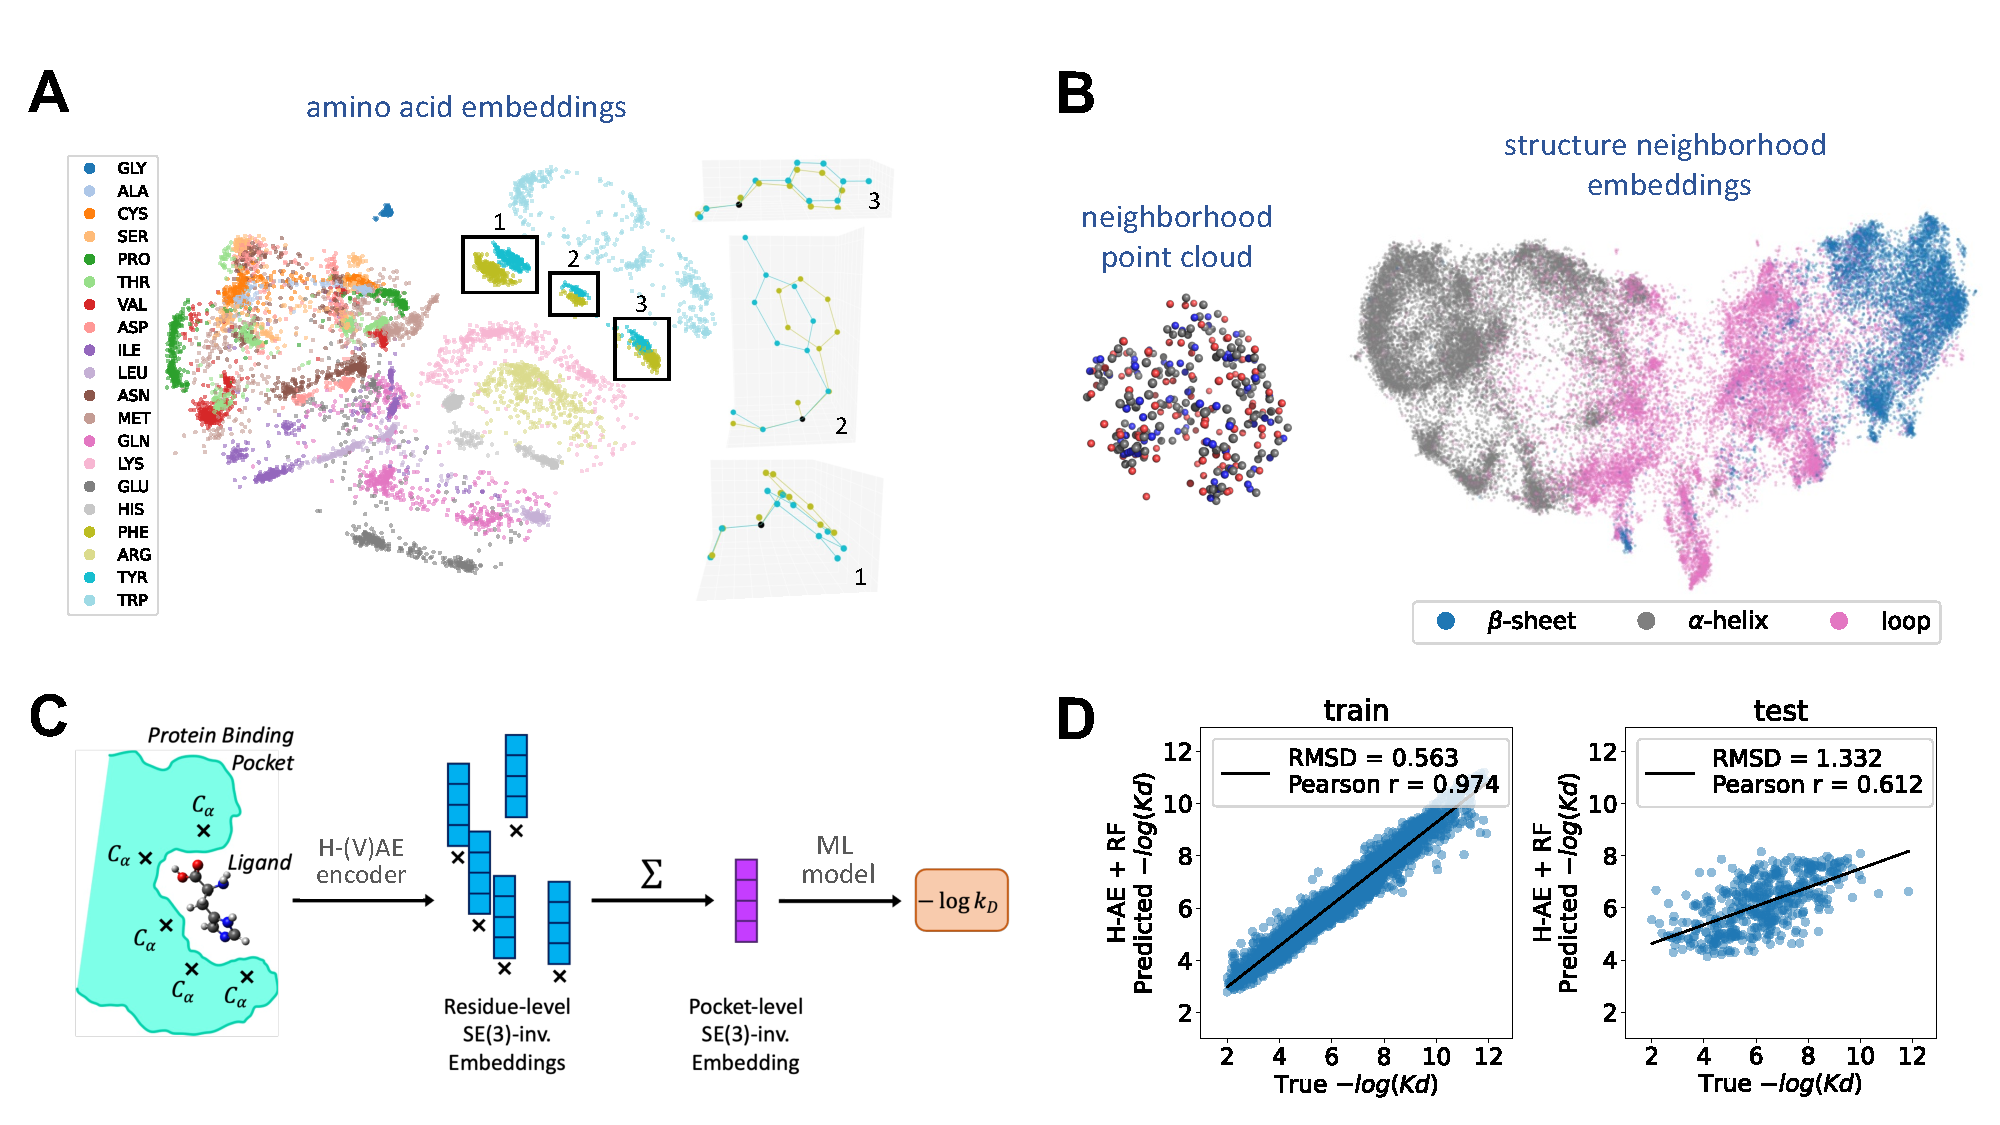
\includegraphics[width=\textwidth]{figures/protein_figure.pdf}\\
    \figcaption{Structural embeddings to predict protein-ligand binding affinities with H-(V)AE.}{
    \textbf{(A)}     H-VAE was trained to reconstruct the Fourier representation of 3D atomic point
    clouds representing amino acids (colors). The invariant latent space clusters by amino acid
    conformations. 
    The highlighted clusters for PHE and TYR contain residue pairs with similar conformations; TYR
    and PHE differ by one oxygen at the end of their benzene rings. We compare conformations by
    plotting each residue in the standard backbone frame (right); $x$ and $y$ axes are set by the
    orthonormalized C$\alpha$-N and C$\alpha$-C vectors, and $z$ axis is their cross product. For
    this plot, 1,000 amino acids were used as training data, with network parameters: $\beta =
    0.025$ and $z = 2$.     
    {\bf (B)} Left: An example protein neighborhood (point cloud of atoms) of 10 \AA\, around a
    central residue, used to train the H-AE models, is shown. Right: 2D UMAP visualization of the
    128-dimensional invariant latent space learned by H-AE trained on the protein structure
    neighborhoods with $L=6$ can separate neighborhoods by the secondary structure of their focal
    amino acid (colors); a linear classifier trained on 300,000 latent embeddings
    predicts secondary struvture of the focal amino-acid with 90\% accuracy. Each point represents
    a neighborhood. See Section~\ref{sec:protein_neighborhoods_details} for details on the
    network architecture and training procedure.
    {\bf (C)}  We use H-AE to extract the residue-level SO(3)-invariant embeddings in the binding
    pocket of a protein-ligand structure complex (data from PDBbind~\cite{su_comparative_2019}). We
    then sum over these embeddings to form an SE(3)-invariant pocket embedding that is used as an
    input to a standard Machine Learning model to predict the  binding affinity between the protein
    and the ligand.
    {\bf (D)} The predictions on the protein-ligand binding affinities from (C) is shown against
    the true values  for the training (left) and the test (right) sets. We use the data split
    provided by ATOM3D~\cite{townshend_atom3d_2021}, which devises training and test sets
    respectively containing 3507, and 490 protein-ligand complexes, with maximum 30\% sequence
    similarly between training and test proteins; see Table~\ref{table:lba_results} for a
    comparison against state-of-the-art methods.}
    \label{fig:lba_diagram}
\end{figure*}


The Shrec17 dataset consists of 51k colorless 3D models belonging to 55 object classes, with a
70/10/20 train/valid/test split~\cite{noauthor_shrec_nodate}. We use the variant of the dataset in
which each object is randomly rotated. Converting 3D shapes into spherical images preserves
topological surface information, while significantly simplifying the representation. We follow
ref.~\cite{cohen_spherical_2018} 
and project surface information for each image onto an enclosing spherical grid via a ray-casting
scheme and apply ZFT (eq.~\ref{eq:ZFT}) on these transformed images.

We train an AE and a VAE model on ZFT transformed data (Section~\ref{sec:shrec17_details}) and,
similarly to the MNIST dataset, compute cosine loss, clustering metrics and classification
accuracy via a linear classifier. We also compute the standard Shrec17 object retrieval metrics via
the latent space linear classifier's predictions (see~\cite{noauthor_shrec_nodate} for a
description of the retrieval metrics). H-AE achieves the best classification and retrieval results
for autoencoder-based models, and is competitive with supervised models despite the lower grid
bandwidth and the small latent space (Table~\ref{table:all_scores}). Using KNN classification
instead of a linear classifier further improves performance
(Table~\ref{table:shrec17_evaluation_knn}). H-VAE achieves slightly worse classification results
but better clustering metrics compared to H-AE. While reconstruction loss is low, there is still
significant margin of improvement. 

\subsection{Structural  embeddings of amino acid neighborhoods to predict function}
Here, we provide a strong use case for H-(V)AE in structural biology. 
Specifically, we learn expressive embeddings for amino acids neighborhoods within protein
structures that can be used to learn protein function.\\

\noindent {\bf \small Embeddings of amino acid conformations.}  As a first, propedeutic step, we
train H-(V)AE to reconstruct the 3D structure of individual amino acids, represented as atomic
point clouds, extracted from protein structures in the Protein Data Bank
(PDB)~\cite{berman_protein_2000}. Residues of the same type have different conformations and
naturally have noisy coordinates, making this problem a natural benchmark for our rotationally
equivariant method. 

We represent an amino acid by atom-type-specific clouds (C, O, N and S; we exclude H) centered at
the residue's C$\alpha$ and compute the ZFT (eq.~\ref{eq:ZFT}) with $L = 4$ and $N = 20$ within a
radius of $10$\AA\, from the residue's C$\alpha$, and concatenate features of the same degree
$\ell$, resulting in a tensor with 940 coefficients. We train several H-AE and H-VAE with different
architectures, but all with the latent space sizes $z=2$; see Sec.~\ref{sec:toy_aminoacids_details}
for details.\\ 


We consistently find that the latent space clusters by amino acid conformations
(Figure~\ref{fig:lba_diagram}A), with sharper cluster separations as more training data is added
(Figure~\ref{fig:toy_aminoacids_data_ablation_umap_AE}
and~\ref{fig:toy_aminoacids_data_ablation_umap_VAE}). We find that test reconstruction loss
decreases with more training data but the reconstruction is accurate even with little training data
(from 0.153 Cosine loss with 400 training residues to 0.034 with 20,000); 
Table~\ref{table:toy_aas_data_ablation_z_eq_2}. A similar trend is observed for KNN-based
classification accuracy of residues (from 0.842 with 400 training residues to 0.972 with 20,000);
(Table~\ref{table:toy_aas_data_ablation_z_eq_2}). Notably, an untrained model, while achieving
random reconstruction loss, still produces an informative invariant latent space (0.629 residue
type accuracy), suggesting that the forced SO(3)-invariance grants a ``warm start" to the encoder.
We do not find significant improvements in latent space classification by training with a
variational objective, and present ablation results in
Table~\ref{table:toy_aas_kld_ablation_z_eq_2}.\\



\noindent {\bf  \small Embeddings of amino acid structure neighborhoods.}  The structural
neighborhood surrounding an amino acid provides a context for its function (e.g., whether it takes
part in interaction with other proteins at a protein-protein interface or not). Indeed, our
previous work has shown that supervised learning algorithms can accurately classify focal amino
acids based on the composition of their surrounding neighborhoods~\cite{pun_learning_2022}. Here,
we  train H-(V)AE to reconstruct residue-specific protein \textit{neighborhoods} - which we define
as the point clouds of atoms within 10\AA\, of a residue's C$\alpha$ - across the protein universe
(Fig.~\ref{fig:lba_diagram}A).  We extract these protein neighborhoods from all proteins in
ProteinNet~\cite{alquraishi_proteinnet_2019}. We then construct each neighborhood's Fourier
representation by computing the ZFT (Eq.~\ref{eq:ZFT}) over the point clouds associated with each
atom type within the neighrbohood (C, N, O and S) and concatenating atom-specific features of the
same degree $\ell$.

We train several H-AE models with varying architectures with different maximum spherical degree $L$
and latent space sizes $z$ (see details in Sec.~\ref{sec:protein_neighborhoods_details}); note that
we do not experiment with variational models for this task. H-AE shows strong reconstruction
ability, but its accuracy worsens with smaller latent space sizes and higher maximum spherical
degree $L$ (Table~\ref{table:mse_and_cosine}).
Notably, the learned latent space is smoothly structured according to geometric
features of the neighborhoods, such as the presence of secondary structure components
(Fig.~\ref{fig:lba_diagram}B and~\ref{fig:umaps_sec_struct_with_abundances}) and number of atoms
(Figure~\ref{fig:umap_total_power}).




\begin{table}[t]
\begin{center}
\resizebox{0.6\textwidth}{!}{
\begin{tabular}{l | c c c}
     & \multicolumn{3}{c}{\newlinecell{\textbf{Ligand Binding Affinity}\\\textbf{30\% Similarity}}}
     \\
    {Model} & {RMSD $\downarrow$} & {Pearson's r $\uparrow$} & {Spearman's r $\uparrow$} \\
    \hline
    DeepDTA &                  $1.565$           & $0.573$           & $0.574$           \\ 
    3DCNN &                    $1.414 \pm 0.021$ & $0.550$           & $0.553$           \\
    GNN &                      $1.570 \pm 0.025$ & $0.545$           & $0.533$           \\
    MaSIF &                    $1.484 \pm 0.018$ & $0.467 \pm 0.020$ & $0.455 \pm 0.014$ \\
    EGNN &                     $1.492 \pm 0.012$ & $0.489 \pm 0.017$ & $0.472 \pm 0.008$ \\
    GBPNet &                   $1.405 \pm 0.009$ & $0.561$           & $0.557$           \\
    EGNN + PLM &               $1.403 \pm 0.013$ & $0.565 \pm 0.016$ & $0.544 \pm 0.005$ \\
    ProtMD  &                  \underline{$1.367 \pm 0.014$} & \underline{$0.601 \pm 0.036$} &
    \underline{$0.587 \pm 0.042$}\\
    \hline
    H-AE + L.R. & $1.397 \pm 0.019$ & $0.560 \pm 0.017$ & $0.568 \pm 0.018$ \\
    H-AE + R.F. &     $\mathbf{1.332 \pm 0.012}$ & $\mathbf{0.612 \pm 0.009}$ & $\mathbf{0.619 \pm
    0.009}$
\end{tabular}
}
\end{center}
    \figcaption{Results on the Ligand Binding Affinity task.}{Prediction accuracies using H-AE
    embeddings with  Linear Regression (L.R.), and  Random Forest (R.F.) Regression are benchmarked
    against other methods. We choose the H-AE model with best RMSD on validation split, which is the
    model with $L = 6$ and $z = 128$ for both Linear Regression and Random Forest. For each set of
    predictions, we use an ensemble of 10 Regressors as we noted a small but consistent improvement
    in performance. Best scores are in \textbf{bold} and second-best scores are \underline{underlined}.
    H-AE+R.F. delivers state-of-the-art predictions. Methods are ordered by date of release;
    see Table~\ref{table:lba_results_appendix} for more details.}
\label{table:lba_results}
\end{table}




\noindent {\bf \small Predicting protein-Ligand Binding Affinity (LBA).}  The binding interaction
between proteins and ligands should be primarily determined  by the composition of the protein's
binding pocket in complex with the ligand. Therefore, we hypothesized that the inferred protein
structure  embeddings  (Fig.~\ref{fig:lba_diagram}B) should contain information about
protein-ligand binding interactions, if the neighborhood is defined along the binding pocket and
contains atoms from the ligand. To test this hypothesis, we  follow the pipeline in
Fig.~\ref{fig:lba_diagram}C. Specifically,  given a protein-ligand structure complex, we identify
residues in the binding pocket (i.e., residues with C-$\alpha$ within 10\AA\, of the ligand) and
extract their structure neighborhoods, which include atoms from both the protein and the ligand. We
then pass the residue-centered neighborhoods of the binding pocket through a trained H-AE's encoder
to extract their rotationally-invariant embeddings. We highlight that, since the neighborhood
centers are well-defined at the residues' C-$\alpha$'s, the embeddings are not only rotationally
invariant about their center, but also translationally invariant with the respect to translations
of the whole system, i.e., they are effectively SE(3)-invariant. 

Since protein-ligand binding affinity is an extensive quantity in the number of interacting
residues, we construct a pocket embedding by summing over residue-level embeddings; the resulting
pocket embedding is SE(3)-invariant, reflecting the natural symmetry of the LBA task. We use these
pocket embeddings as feature vectors to train simple Machine Learning models to predict
protein-ligand binding affinities. 


To test the performance of our method, we use the LBA dataset in
ATOM3D~\cite{townshend_atom3d_2021} that provides the PDB structure of the protein-ligand complex
together with   either the measured dissociation constant $K_d$ or the inhibition constant $K_i$;
see Sec.~\ref{sec:lba_details} for further details. To map between the learned pocket embeddings to
the log dissociation (or inhibition) constants we train both a simple Linear and a Random Forest
Regressor on a training sets provided by ATOM3D.  Fig.~\ref{fig:lba_diagram}D shows the performance
of the model with the Random Forest Regressor and Table~\ref{table:lba_results} provide a detailed
benchmark of our methods against prior approaches.  The Linear model achieves competitive results,
whereas the Random Forest Regressor achieves state-of-the-art. 

These results demonstrate the utility of unsupervised learning for residue-level protein structure
representations in predicting complex protein functions. Most of the competing structure-based
methods for LBA (Table~\ref{table:lba_results}) learn complex graph-based functions on top of
simple atomic representation, whereas our method uses simpler machine learning models over rich
residue-level representations. Notably, ProtMD (the method competitive to ours) performs a
pre-training scheme using expensive molecular dynamics simulations that informs the model about
conformational flexibility, information that our method does not have access to. Given the
computational cost of training complex atom-level graph-based models, our residue-based approach
can offer a more viable alternative for modeling large protein interfaces.


\section{Summary}

In this chapter, we have developed the first end-to-end SO(3)-equivariant unsupervised algorithm, termed Holographic
(Variational) Auto-Encoder (H-(V)AE), suitable for data distributed in three dimensions around a given central point.
The model learns an invariant embedding describing the data in a ``canonical" orientation alongside an equivariant frame
describing the data's original orientation relative to the canonical one.

Prior works have attempted to learn representations that are invariant to certain transformations. For example, in
refs.~\cite{shu_deforming_2018, koneripalli_rate-invariant_2020} general ``shape" embeddings are learned by
characterizing a separate ``deformation" embedding. However, these networks are not explicitly equivariant to the
transformations of interest.

Others proposed to learn an exactly invariant embedding alongside an approximate (but not equivariant) group action to
align the input and the reconstructed data. For example, {\em Mehr et al}~\cite{mehr_manifold_2018} learns in
quotient space by pooling together the latent encodings of copies of the data that have been transformed with sampled
group actions, and backpropagate the minimum reconstruction loss between the decoded element and the transformed copies
of the data. This approach is best suited for discrete and finite groups, for which it does not require approximations,
and it is computationally expensive as it is akin to data augmentation. {\em Lohit et
al}~\cite{lohit_rotation-invariant_2020} construct an SO(3)-invariant autoencoder for spherical signals by learning an
invariant latent space and minimizing a loss which first finds the rotation that best aligns the true and reconstructed
signals. Although this approach is effective for non-discrete data, it still manually imposes rotational invariance, and
can only reconstruct signals up to a global rotation. In contrast, H-(V)AE is fully equivariant and only requires simple
MSE for reconstruction of data in its original orientation.

A small body of work went beyond invariance to develop equivariant autoencoders. Several methods construct data and
group-specific architectures to auto-encode data equivariantly, learning an equivariant representation in the
process~\cite{hinton_transforming_2011, kosiorek_stacked_2019}. Others use supervision to extract class-invariant and
class-equivariant representations~\cite{feige_invariant-equivariant_2022}. A recent theoretical work proposes to train
an encoder that encodes elements into an invariant embedding and an equivariant group action, then using a standard
decoder that uses the invariants to reconstruct the elements in a canonical form, and finally applying the learned group
action to recover the data's original form~\cite{winter_unsupervised_2022}. Our method in SO(3) is closely related to
this work, with the crucial difference that our network is end-to-end rotationally equivariant, in that we use an
equivariant decoder and learn to reconstruct the Fourier encoding of the data. A more detailed comparison of the two
approaches and the benefits of our fully equivariant approach can be found in the Appendix
(Section~\ref{sec:mlp_decoder_appendix}) and in Table~\ref{table:mlp_decoder_comparison}.
Recently, generative models of atomic point clouds that are equivariant to Euclidean transformation have been developed
for molecular~\citep{hoogeboom_equivariant_2022} and protein~\citep{yim_se3_2023, watson_broadly_2022} generation in
3D using Normalizing Flows~\citep{hoogeboom_equivariant_2022} and diffusion processes~\citep{satorras_en_2022,
yim_se3_2023, watson_broadly_2022}. Our work is partly related to these, but with some crucial differences. 1) Our
method is designed for spherical images and for point clouds with a preferential center, as opposed to point clouds. 2)
The use of an autoencoder architecture makes our method suitable for compressing information into a lower-dimensional
space, for effective later use in annotation-scarce domains like ligand binding affinity prediction; by contrast the
latent space of normalizing flows and diffusion-based models must have the same size as the data, making them unsuitable
for this task.

There is also a diverse body of literature on constructing representations of atomic systems that are
invariant/equivariant to euclidean symmetries, leveraging Fourier transforms and CG tensor products, with focused
applications on materials science~\cite{drautz_atomic_2019, musil_physics-inspired_2021, uhrin_through_2021}\\

H-(V)AE's learned embeddings are highly expressive. For example, we used the learned invariants to achieve
state-of-the-art unsupervised clustering and classification results on various spherical image datasets. By making our
model variational in its invariant latent space, we enhanced the quality of clustering and made the model generative.
Our model is defined fully in spherical Fourier space, and thus, can reach a desired expressiveness without a need for
excessive computational resources.

H-(V)AE also produces rich residue-level representations of local neighborhoods in protein structures, which we use as
embeddings for downstream structure-based tasks such as Ligand Binding Affinity prediction. Indeed, H-(V)AE
representations paired with a simple Random Forest Regressor achieve state-of-the-art results on learning the binding
affinity between proteins and small molecule ligands.

More broadly, we expect that H-(V)AE can be used to extract rich, symmetry-aware features from local neighborhoods in
spherical images and complex 3D objects, to be used in more complex downstream tasks that benefit from the symmetry
constraints. For example, our method can be leveraged for modeling diffusion MRI data, for which rotation-equivariant
methods have recently shown to be highly beneficial~\cite{muller_rotation-equivariant_2021}. In structural biology, we
expect our method to be useful for coarse-graining full-atom representations of protein structures to facilitate
structure-based predictions of protein function. For example, a large protein graph can be coarse-grained by
substituting its full-atom representation with rich embeddings of local structural neighborhoods learned from an
unsupervised model. With an added supervised step, these coarse-grained embedding can be leveraged to predict complex
protein functions, as we show for predicting ligand binding affinity. This approach is akin to using protein
embeddings for sequence data, learned by language models, to inform (few-shot) predictions for protein
function~\cite{swanson_predicting_2022}.


